\documentclass[]{article}
\usepackage{amssymb,amsmath}
\usepackage{hyperref}

\usepackage{todonotes}
\usepackage[margin=2.5cm]{geometry}
\usepackage[super]{natbib}
\bibliographystyle{unsrtnat}


\title{INFORMATION THEORY AND STATISTICAL MECHANICS}

\author{E. T. JAYNES\\
Washington University}


\begin{document}

BRANDEIS UNIVERSITY SUMMER INSTITUTE\\
LECTURES IN THEORETICAL PHYSICS

K. W. Ford, \emph{\textbf{Editor}}

\begin{enumerate}
\def\labelenumi{\arabic{enumi}.}
\setcounter{enumi}{1959}
\item
  Lectures
\end{enumerate}

\begin{quote}
C. Miller • P. T. Matthews • J. Schwinger • N. Fukuda • J. J. Sakurai
\end{quote}

\begin{enumerate}
\def\labelenumi{\arabic{enumi}.}
\setcounter{enumi}{1960}
\item
  \begin{quote}
  Lectures\emph{\textbf{Vol. l}}
  \end{quote}
\end{enumerate}

\begin{quote}
R. J. Eden • J. C. Polkinghorne • G. Källén • J. J.Sakurai
\end{quote}

\emph{\textbf{Vol. 2}}

\begin{quote}
M. E. Rose • E, C. G. Sudarshan
\end{quote}

\begin{enumerate}
\def\labelenumi{\arabic{enumi}.}
\setcounter{enumi}{1961}
\item
  Lectures
\end{enumerate}

\begin{quote}
\emph{\textbf{Vol 1---Elementary Particle Physics and Field Theory}} T.
Fulton • G. Kallen • J. D. Jackson • C. Fronsdal

\emph{\textbf{Vol 2---Astrophysics and ihe Many-Uody Problem}} E. N,
Parker • J. S. Goldstein • A, A. Maiadudin •V. Anibcgaokar

\emph{\textbf{VoL 3---Statistical Physics}} G. E. Uhlenbeck • N.
Rosenzwcig • A. J. F Siegcrt •

E, T. Jaynes • S. Fujita
\end{quote}

Brandeis Summer Institute 1962

STATISTICAL

PHYSICS

3

G. E. Uhlenbeck N. Hosenzweig A, J, F. Siegert E. T. Jaynes S. Fujita

\emph{\textbf{W. A.}} BENJAMIN, INC\emph{\textbf{.}} STATISTICAL PHYSICS

\begin{quote}
1962 Brandeis Lectures in Theoretical Physics, Volume 3

G. E. Uhlenbeck, N. Rosenzweig, A. J. F. Siegert, E. T. Jaynes, and C.
Fujita.
\end{quote}

In his course on SELECTED TOPICS IN STATISTICAL MECHANICS, Professor G.
E. Uhlenbeck begins with an exposition of some diagrammatic methods used
to calculate virial coefficients and the equation of state. He then
gives a detailed analysis of the mathematics of phase transition with a
soluble one-dimensional model.

The second set of lectures, by Dr. N. Rosenzweig, STATISTICAL MECHANICS
OF EQUALLY LIKELY QUANTUM SYSTEMS, is a discussion of the statistical
properties of energy levels and eigenfunctions for heavy nuclei and
complex atoms, stressing the role of time reversal and other symmetries.

Professor A. J. F. Siegert lectures on FUNCTIONAL INTEGRALS IN
STATISTICAL MECHANICS, demonstrating the utility of new techniques by
analysis of the partition function of the Ising model with long range
interactions.

Information theory has provided the long hoped for algorithm analogous
to the partition sum of equilibrium theory, for calculation of
irreversible processes. The lectures of Professor E. T. Jaynes,
INFORMATION THEORY AND STATISTICAL MECHANICS, provide an introduction to
this subject.

In the final set of lectures, Professor C. Fujita reviews and compares
the independent achievements of Van Hove and Prigogine and their
schools, in their progress toward better understanding the APPROACH TO
EQUILIBRIUM OF A MANY-PARTICLE SYSTEM.





\section*{Foreword}

It is now an established tradition of the Brandeis Summer Institute in
Theoretical Physics to have lecturers who present a systematic account
of recent research in various fields of theoretical physics. The lecture
notes have also become a part of tins tradition, and, although these are
sometimes but a first approximation to the spoken lecture, they may
serve to bring these much needed expositions to the wider audience of
physicists who may aspire to contribute to these fields.

I should like to take this opportunity to thank all those whose
participation in the Institute during the summer of 1962 helped maintain
these traditions. Particular words of appreciation are due the National
Science Foundation, for its indispensable financial support, and
Professor Kenneth Ford, who graciously carried the responsibility for
getting the notes ready for publication.

In this volume, the notes of Professor Jaynes and Professor Fujita have
been prepared by the lecturers; Professor Uhlenbeck, Dr. Rosenzweig, and
Professor Siegert have kindly checked over the notes based on their
lectures.

\begin{quote}
\emph{\textbf{\textsc{David L. Falkoff}}} Co-Director of the
\emph{\textbf{1962}} Institute

\maketitle 

Notes by the lecturer

\tableofcontents

\section{Introduction}\label{introduction}

At the beginning of every problem in probability theory, there arises a
need to assign some initial probability distribution; or what is the
same thing, to ``set up an ensemble.'' This is a problem which cannot be
evaded, and for which the laws of physics give us no help. For example,
the laws of physics tell us that a density matrix
\(\rho\left( t \right)\) must vary with time according to
\(\dot{\rho} = \lbrack H,\rho\rbrack}\), but they do not
tell us what function \(\rho(0)\) should be put in at the start.
Assignment of \(\rho(0)\) is, of course, a matter of free choice on our
part---it is for us to say which problem we want to solve.

The assignment of initial probabilities must, in order to be useful,
agree with the initial information we have (i.e., the results of
measurements of certain parameters). For example, we might know that at
time \(t = 0\), a nuclear spin system having total (measured) magnetic
moment \(M(0)\), is placed in a magnetic field \(H\), and the problem is
to predict the subsequent variation \(M(t)\), which presumably tends to
an equilibrium value \(M\left( \infty \right) = x_{0}H\) after a long
time. What initial density matrix for the spin system \(\rho(0)\),
should we use? Evidently, we shall want it to satisfy, at the very
least,

\begin{equation}
\text{Tr}\left( \rho(0)M_{o_{p}} \right) = M(0) \label{eqn-one}
\end{equation}

where \(M_{o_p}\) is the operator corresponding to total magnetic moment. But Eq. (\ref{eqn-one}) is very far from uniquely
specifying \(\rho(0)\). Out of the infinite number of density matrices
satisfying (\ref{eqn-one}), which should we choose as the starting point of our
calculation to predict \(M(t)\)?

Conventional quantum theory has provided an answer to the problem of
setting up initial state descriptions only in the limiting case where
measurements of a ``complete set of commuting observables'' have been
made, the density matrix \(\rho(0)\) then reducing to the projection
operator onto a pure state \(\psi(0)\) which is the appropriate
simultaneous eigenstate of all the measured quantities. But there is
almost no experimental situation in which we really have all this
information, and before we have a theory able to treat actual
experimental situations, existing quantum theory must be supplemented
with some principle that tells us how to translate, or encode, the
results of measurements into a definite state description \(\rho(0)\).
Note that the problem is not to find the \(\rho(0)\) which correctly
describes the "true physical situation." That is unknown, and always
remains so, because of incomplete information. In order to have a usable
theory we must ask the much more modest question: ``What \(\rho(0)\) best
describes our \emph{state of knowledge} about the physical situation?''

In order to emphasize that this problem really has nothing to do with
the laws of physics (and, as a corollary, that its solution will have
applications outside the field of physics), consider the following
problem. A die has been tossed a very large number \(N\) of times, and
we are told that the \emph{average} number of spots up per toss was not
3.5, as we might expect from an honest die, but 4.5. Translate this
information into a probability assignment
\(P_{n},n = 1,\ 2,\ \ldots,6\), for the \(n\)th face to come up on the
next toss.

To explain more fully what is meant by this, note that we are not asking
for an estimate of the fraction (i.e., the relative frequency) of tosses
which give \(n\) spots There is, indeed, a connection between the
probability and the frequency, which we will derive later. But the
problem stated is to reason as best we can about the \emph{individual}
case. The probability \(P_{n}\) must therefore be interpreted in the
so-called "subjective" sense; it is only a means of describing how
strongly we \emph{believe} that the \(n\)-th face will come up in the
next toss.

To state the problem more drastically, imagine that we are offered
several bets, at various odds, on various values of \(n\), and we are
compelled to accept one of these bets. The probabilities \(P_{n}\) are
the basic raw material from which we decide which one to accept. This is
typical of many practical problems faced by the scientist, the engineer,
the statistician, the politician; and indeed all of us. We are
continually faced with situations where some definite decision must be
made \emph{now}, even though we do not have all the information we might
like.

\begin{align}
\sum_{n = 1}^{6} P_{n} = & 1  \label{eqn-two} \\
\sum_{n = 1}^{6} nP_{n} = & 4.5 \label{eqn-three}
\end{equation}

\begin{figure}
    \centering
    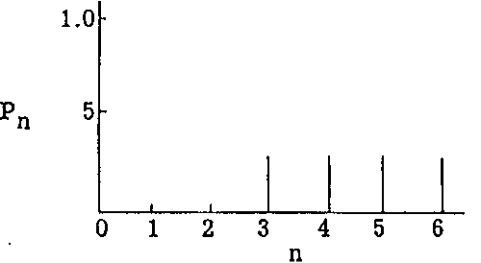
\includegraphics[width=3.20866in,height=1.75197in]{media/image1.jpeg}
    \caption{}
    \label{fig-one}
\end{figure}

\begin{figure}
    \centering
    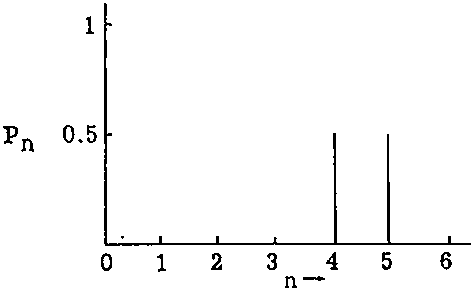
\includegraphics[width=3.16142in,height=2in]{media/image2.png}
    \caption{}
    \label{fig-two}
\end{figure}

}where
(\ref{eqn-three}) is analogous to (\ref{eqn-one}). A possible solution of (\ref{eqn-two}) and (\ref{eqn-three}) is indicated
in Fig. \ref{fig-one}; we could take \(P_{4} = P_{5} = 1/2\), all other
\(P_{n} = 0\), This agrees with all the given data. But our common sense
tells us it is not a \emph{reasonable} assignment. The assignment of
Fig. \ref{fig-two} is evidently a more honest description of what we know. But even
this is not reasonable---nothing in the data tells us that n = 1, 2 are
impossible events. In Fig. \ref{fig-two}, we are still jumping to conclusions not
warranted by the available evidence. Evidently, it is unreasonable to
assign probability zero to any situation unless our data really rules
out that case. If we assign \(P_{1} > 0\), \(P_{2} > 0\), then in order
to keep the average at 4.5, we shall have to give some increased weight
to the cases \(n = 5,\ 6\). Figure \ref{fig-three} shows an assignment that agrees
with the data and does not ignore any possibility. But it still seems
unreasonable to give the case \(n = 6\) such exceptional treatment.
Figure \ref{fig-four} represents what we should probably call a
\begin{figure}
    \centering
    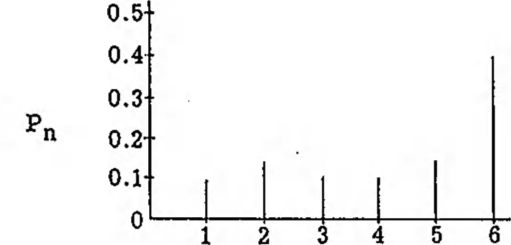
\includegraphics[width=3.39764in,height=1.64567in]{media/image3.jpeg}
    \caption{}
    \label{fig-three}
\end{figure}
\begin{figure}
    \centering
    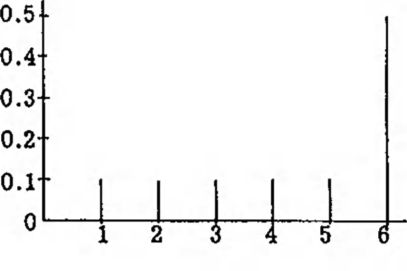
\includegraphics[width=2.71319in,height=1.81042in]{media/image4.jpeg}
    \caption{}
    \label{fig-four}
\end{figure}
backward
step---nothing in the data of the problem indicates any reason for such
an uneven treatment. A reasonable assignment \(P_{n}\) must not only
agree with the data and must not ignore any possibility---but
it must also not give undue emphasis to any possibility. The \(P_{n}\)
should vary as smoothly as possible, in some sense. One criterion of
"smoothness" might be that adjacent differences \(P_{n + 1} - P_{n}\)
should be constant; and, indeed, there is a solution with that property.
It is given by \(P_{n} = (12n - 7)/210\) and
\begin{figure}
    \centering
    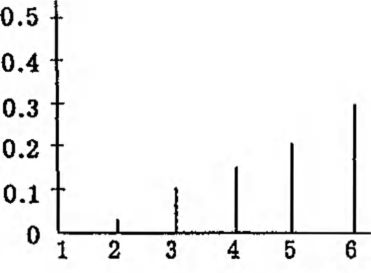
\includegraphics[width=2.48031in,height=1.82283in]{media/image5.jpeg}
    \caption{}
    \label{fig-five}
\end{figure}
is
shown in Fig. \ref{fig-five}. This is evidently the most reasonable probability
assignment so far. But there is a limit to how high an average you can
get with this linear variation of \(P_{n}\). If we took the extreme
case, \(P_{n} = (const.)(n - 1)\), we should again violate one of our
principles because \(P_{1} = 0\), and the average would be only
\(\sum_{n}^{}{P_{n} = 70/15} = 4.67\). Suppose the data of the problem
had been changed so that the average is to be 4.7 instead of 4.5. Then
there is no straight-line solution satisfying \(P_{n} \geq 0\). The
\(P_{n}\) must lie on some concave curve, as in Fig. 6. But the
principles by which we reason
surely
\begin{figure}
    \centering
    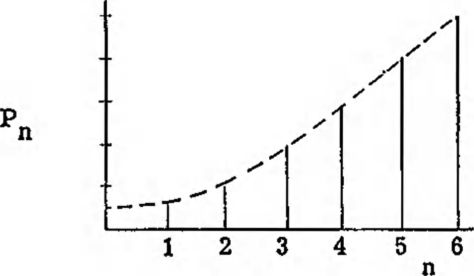
\includegraphics[width=3.16535in,height=1.84252in]{media/image6.jpeg}
    \caption{}
    \label{fig-six}
\end{figure}
%
are the same whether the data specify 4.5 or 4.7; so it appears that a
result qualitatively such as Fig. \ref{fig-six} should be used also when
\(n = 4.5\).

This is about as far as qualitative reasoning can take us, and I have carried the argument through on that basis in order to show how ordinary common sense leads us to a result that has all the important features of the quantitative solution given below. The probability assignment $P _{ n }$ which most honestly describes what we know is the one that is as smooth and "spread out" as possible subject to the data. It is the most conservative assignment in the sense that it does not permit one to draw any conclusions not warranted by the data.

This suggests that the problem is a variational one; we need a measure of the "spread" of a probability distribution which we can maximize, subject to constraints which represent the available information. It is by now amply demonstrated by many workers that the "information measure" introduced by Shannon' has special properties of consistency and uniqueness which make it \emph{the} correct measure of "amount of uncertainty" in a probability distribution. This is, of course, the expression
%
\begin{equation}
S_{I} = - \sum_{i}^{} p_{i}\log p_{i}
\end{equation}
%
which, \emph{for some distributions} and \emph{in some physical situations}, has long been recognized as representing entropy. However, we have to emphasize that "information-theory entropy" $S _{ I }$ and the experimental thermodynamic entropy $S _{e}$ are entirely different concepts. Our job cannot be to \emph{postulate} any relation between them; it is rather to \emph{deduce} whatever relations we can from known mathematical and physical facts. Confusion about the relation between entropy and probability has been one of the main stumbling blocks in developing a general theory of irreversibility.

\section{The General Maximum-Entropy Formalism}\label{the-general-maximum-entropy-formalism}

To generalize the above problem somewhat, suppose that the quantity
\(x\) can take on the values \((x_1, x_2, \dots x_n)\) where $n$ can be finite or
infinite, and that the average values of several functions $(f_1(x), f_2(x), \dots f_m(x)$ are given, where $m < n$. The problem is to find the probability assignment $p_i =
p(x_i)$ which satisfies the given data: $p_i \geq 0$,
%
\begin{equation}
\sum_{i = 1}^{n} p_{i} = 1 \label{eqn-five}
\end{equation}
\begin{equation}
\sum_{i = 1}^{n}  p_{i}f_{k}\left( x_{i} \right) = \left\langle f_{k}(x) \right\rangle = F_{k} \quad k = 1,2,\ldots,m \label{eqn-six}
\end{equation}
%
and, subject to (\ref{eqn-five}) and (\ref{eqn-six}), maximizes the entropy
%
\begin{equation}
S_{I} = - \sum_{i = 1}^{n} p_{i}\log p_{1}
\end{equation}
%
The solution to this mathematical problem can be found immediately by
the method of Lagrangian multipliers, and special cases are given in
every statistical mechanics textbook. This method has the merit that it
leads immediately to the answer, but the weakness that it does not make
it obvious whether one obtains a true absolute maximum of \(S_{I}\). The
following argument establishes this important result more rigorously.
Let \(\left( p_{1}\ldots p_{n} \right)\) and
\(\left( u_{1}\ldots u_{n} \right)\) be any two possible probability
distributions over the \(x_{1};\) i.e.,
\(p_{i} \geq 0,u_{i} \geq 0,i = 1,2,\ldots\) n and
%
\begin{equation}
\sum_{i = 1}^{n} p_{1} = \sum_{i = 1}^{n} u_{i} = 1
\end{equation}
%
Then, by using the fact that
\(logx \geq \left( 1 - x^{- 1} \right),\) with equality if and only if
\(x = 1,\) we find the following:

\paragraph{Lemma}

\begin{equation}
\sum_{i = 1}^{n}  p_{i}\log\frac{p_{i}}{u_{i}} \geq \sum_{i = 1}^{n}  p_{i}\left( 1 - \frac{u_{i}}{p_{i}} \right) = 0
\end{equation}
%
with equality if and only if \(p_{i} = u_{i},i = 1,2,\ldots n\). Now
make the choice
%
\begin{equation}
u_{i} = \frac{1}{Z\left( \lambda_{1}\ldots\lambda_{m}) \right.\ }\exp\left( - \lambda_{1}f_{1}\left( x_{i} \right) - \ldots - \lambda_{m}f_{m}\left( x_{i} \right) \right)
\end{equation}
%
where \(\lambda_{1}\ldots\lambda_{m}\) are fixed constants, and
%
\begin{equation}
Z\left( \lambda_{1}\ldots\lambda_{m} \right) \equiv \sum_{i = 1}^{n}  \exp\left( - \lambda_{1}f_{1}\left( x_{1} \right) - \ldots - \lambda_{m}f_{m}\left( x_{i} \right) \right)
\end{equation}
%
will be called the ``partition function.'' Substituting (10) into (9)
results in the inequality

\begin{align*}
\sum_{i = 1}^{n}   p_{i}\log p_{i} \geq \sum_{i = 1}^{n}   p_{i}\log u_{i} = &  - \sum_{i = 1}^{n}   p_{i}\left\lbrack \lambda_{1}f_{1}\left( x_{i} \right) + \ldots \right. \\
 & \left.  + \lambda_{m}f_{m}\left( x_{i} \right) \right\rbrack - \log Z\left( \lambda_{1}\ldots\lambda_{m} \right) \\
\end{align*}

or

\begin{equation}s_{1} \leq  \log Z\left( \lambda_{1}\ldots\lambda_{m} \right) + \sum_{k = 1}^{m} \lambda_{k}\left\langle f_{k} \right\rangle\end{equation}

Now let the distribution \(p_{1}\) vary over the class of all possible
distributions that satisfy (6). The right-hand side of (12) remains
fixed, and (12) shows that \(S_{1}\) attains its maximum possible value
%
\begin{equation}\left( S_{I} \right)_{\max} =  \log Z + \sum_{k = 1}^{m} \lambda_{k}\left\langle f_{k} \right\rangle\end{equation}
%
if and only if \(p_{i}\) is taken as the generalized canonical
distribution\\
(10). It only remains to choose the unspecified constants
\(\lambda_{k}\) so that (6) is satisfied. This is the case, as one
readily verifies, if the \(\lambda_{k}\) are determined in terms of the
given data \(F_{k} = \left\langle f_{k} \right\rangle\) by

\begin{equation}\left\langle f_{k} \right\rangle = - \frac{\partial}{\partial\lambda_{k}} \log Z\left( \lambda_{1}\ldots\lambda_{m} \right)\ k = 1,2,\ldots,m\end{equation}

We now survey rapidly the main formal properties of the distribution
found. The maximum attainable entropy (13) is some function of the given
data:

\begin{equation}\left( S_{I} \right)_{\max} = S\left( \left( f_{2} \right),\ldots\left\langle f_{m} \right\rangle \right)\end{equation}

and, by using (13) and (14), we find

\begin{equation}\frac{\partial S}{\partial\left\langle f_{k} \right\rangle} = \lambda_{k}\ k = 1,2,\ldots,m\end{equation}

Regarding, in (14), the \(\left\langle f_{k} \right\rangle\) expressed
as functions of \(\left( \lambda_{1}\ldots\lambda_{m} \right)\) we find,
on differentiating, the reciprocity law

\begin{equation}\frac{\partial\left\langle f_{k} \right\rangle}{\partial\lambda_{j}} = \frac{\partial\left\langle f_{j} \right\rangle}{\partial\lambda_{k}} = - \frac{\partial^{2}}{\partial\lambda_{k}\partial\lambda_{j}} \log Z = A_{\text{jk}}\end{equation}

while by the same argument, if we regard \(\lambda_{k}\) in (16)
expressed as

a function of
\(\left\langle f_{1} \right\rangle\ldots\left\langle f_{m} \right\rangle,\)
we find a corresponding law

\begin{equation}\frac{\partial\lambda_{k}}{\partial\left\langle f_{j} \right\rangle} = \frac{\partial\lambda_{j}}{\partial\left\langle f_{k} \right\rangle} = \frac{\partial^{2}S}{\partial\left\langle f_{j} \right\rangle\partial\left\langle f_{k} \right\rangle} = B_{\text{jk}}\end{equation}

Comparing (17) and (18) and remembering the chain rule for
differentiating,
%
\begin{equation*}
\frac{\partial\left\langle f_{j} \right\rangle}{\partial\left\langle f_{k} \right\rangle} = \sum_{ \ell}^{} \frac{\partial\left\langle f_{j} \right\rangle}{\partial\lambda_{ \ell}}\frac{\partial\lambda_{ \ell}}{\partial\left\langle f_{k} \right\rangle} = \delta_{jk}
\end{equation*}
%
we see that the second derivatives of \(S\) and of $\log Z$ yield
inverse matrices:

\begin{equation}A = B^{- 1}\end{equation}

The functions \( \log Z\left( \lambda_{1}\ldots\lambda_{n} \right)\) and
\(S\left( \left\langle f_{1} \right\rangle\ldots\left\langle f_{n} \right\rangle \right)\)
are equivalent in the sense that each gives full information about the
probability distribution; indeed (13) is just the Legendre
transformation that takes us from one representative function to the
other.

The reciprocity law (17) acquires a deeper meaning when we consider the
``fluctuations'' in our probability distribution. Using the distribution
(10), a short calculation shows that the second central moments of the
distribution of the \(f_{k}(x)\) are given by

\begin{align}
\left\langle \left( f_{k} - \left\langle f_{k} \right\rangle \right)\left( f_{ \ell} - \left\langle f_{ \ell} \right\rangle \right) \right\rangle = \left\langle f_{k}f_{ \ell} \right\rangle & \  - \left\langle f_{k} \right\rangle\left\langle f_{ \ell} \right\rangle \nonumber \\
& \\
 = & \frac{\partial^{2}}{\partial\lambda_{k}\partial\lambda_{ \ell}} \log Z \nonumber
\end{align}

and so, comparing with (17) , there is a universal relation between the
``fluctuations'' of the \(f_{k}\) and the ``compliance coefficients''
\(\partial\left\langle f_{k} \right\rangle/\partial\lambda_{ \ell}:\)

\begin{equation}\left\langle f_{k}f_{l} \right\rangle - \left\langle f_{k} \right\rangle\left\langle f_{ \ell} \right\rangle = - \frac{\partial\left\langle f_{k} \right\rangle}{\partial\lambda_{ \ell}} = - \frac{\partial\left\langle f_{ \ell} \right\rangle}{\partial\lambda_{k}}\end{equation}

Likewise, higher derivatives of
\( \log Z\left( \lambda_{1}\ldots\lambda_{n} \right)\) yield higher central
moments of the \(f_{k}\), in a manner analogous to (20), and a hierarchy
of fluctuation laws similar to (21).

In addition to their dependence on \(x\), the functions \(f_{k}\) may
depend on another parameter, \(\alpha.\) The partition function will
then also have an explicit dependence on \(\alpha\) :
%
\begin{equation}
Z\left( \lambda_{1}\ldots\lambda_{m};\alpha \right) \equiv \sum_{i = 1}^{n}  exp\left( - \lambda_{1}f_{1}\left( x_{i};\alpha \right) - \ldots - \lambda_{m}f_{m}\left( x_{i};\alpha \right) \right)
\end{equation}
%
and a short calculation shows that the expected derivatives
%
\begin{equation*}
\left\langle \frac{\partial f_{k}}{\partial\alpha} \right\rangle
\end{equation*}
%
satisfy the relations
%
\begin{equation}\sum_{k = 1}^{m} \lambda_{k}\left\langle \frac{\partial f_{k}}{\partial\alpha} \right\rangle = - \frac{\partial}{\partial\alpha} \log Z = - \frac{\partial S}{\partial\alpha}\end{equation}
%
If several parameters \(\alpha_{1}\ldots\alpha_{r}\) are present, a
relation of this form will hold for each of them.

Finally, we note an important variational property which generalizes
(16) to the case where we have also variations in the parameters
\(\alpha_{1}\ldots\alpha_{r}.\) Let
\(Z = Z\left( \lambda_{1}\ldots\lambda_{m};\alpha_{1}\ldots\alpha_{r} \right),\)
and consider an arbitrary small change in the problem, where the given
data \(\left\langle f_{k} \right\rangle\) and the parameters
\(\alpha_{j}\) are changed by small amounts
\(\delta\left\langle f_{k} \right\rangle/\delta\alpha_{j}\) This will
lead to a change \(\delta\lambda_{k}\) in \(\lambda_{k}\). From (13),
the maximum attainable entropy is changed by

\begin{align}
\delta S = & \sum_{k = 1}^{m}  \frac{\partial  \log Z}{\partial\lambda_{k}}\delta\lambda_{k} + \sum_{j = 1}^{r}  \frac{\partial  \log Z}{\partial\alpha_{j}}\delta\alpha_{j} \nonumber \\
\\
 & \  + \sum_{k = 1}^{m}  \left\langle f_{k} \right\rangle\delta\lambda_{k} + \sum_{k = 1}^{m}  \lambda_{k}\delta\left\langle f_{k} \right\rangle \nonumber
\end{align}

The first and third terms cancel by virtue of (14). Then, using (23), we
have
%
\begin{equation}
\delta S = - \sum_{j = 1}^{r} \sum_{k = 1}^{m} \lambda_{k}\left\langle \frac{\partial f_{k}}{\partial\alpha_{j}} \right\rangle\delta\alpha_{j} + \sum_{k = 1}^{m} \lambda_{k}\delta\left\langle f_{k} \right\rangle
\end{equation}
%
Now we can write
%
\begin{equation}
\sum_{j = 1}^{r} \left\langle \frac{\partial f_{k}}{\partial\alpha_{j}} \right\rangle\delta\alpha_{j} = \left\langle \sum_{j = 1}^{r}  \frac{\partial f_{k}}{\partial\alpha_{j}}\delta\alpha_{j} \right\rangle = \left\langle \delta f_{k} \right\rangle
\end{equation}
%
and so finally
%
\begin{equation}\text{δS} = \sum_{k = 1}^{m} \lambda_{k}\left\lbrack \delta\left( f_{k} \right\rangle - \left\langle \delta f_{k} \right\rangle \right\rbrack\end{equation}
%
or
%
\begin{equation}\text{δS} = \sum_{k = 1}^{m} \lambda_{k}\delta Q_{k}\end{equation}
%
where
%
\begin{equation}
\delta Q_{k} \equiv \delta\left\langle f_{k} \right\rangle - \left\langle \delta f_{k} \right\rangle
\end{equation}

In general \(\delta Q_{k}\) is not an exact differential; i.e., there is
no function
\(Q_{k}\left( \lambda_{1}\ldots\lambda_{m};\alpha_{1}\ldots\alpha_{r} \right)\)
which yields \(\delta Q_{k}\) by differentiation. But (28) shows that
\(\lambda_{k}\) is an integrating factor such that
\(\sum_{k} \lambda_{k}\delta Q_{k}\) is the exact
differential of some ``state function''
\(S\left( \lambda_{1}\cdots\lambda_{m};\alpha_{2}\cdots\alpha_{r} \right)\).

All the above relations, (10) to (29), are elementary consequences of
maximizing the information theory entropy subject to constraints on
average values of certain quantities. Although they bear a strong formal
resemblance to the rules of calculation provided by statistical
mechanics, they make no reference to physics, and, therefore, they must
apply equally well to any problem, in or out of physics, where the
situation can be described by (1) enumerating a discrete set of
possibilities and by (2) specifying average values of various
quantities. The above formalism has been applied also to problems in
engineering\citep{Jaynes-decipherability59} and economics.\citep{Jaynes-engineering63}

In most problems, interest centers on making the best possible
predictions for a \emph{specific} situation, and we are not really
interested in properties of any ensemble, real or imaginary. (For
example, we want to predict the magnetization \(M(t)\) of the
\emph{particular} spin system that exists in the laboratory.) In this
case, as already emphasized, the maximum-entropy probability assignment
\(p_{i}\) cannot be regarded as describing any objectively existing
state of affairs; it is only a means of describing a state of knowledge
in a way that. is ``maximally noncommital'' by a certain criterion.

The above equations then represent simply the best predictions we are
able to make on the given information. We are not entitled to assert
that the predictions must be ``right,'' only that to make any better
ones, we should need more information than was given. However, in cases
where it makes sense to imagine \(x_{i}\) as being the result of some
random experiment which can be repeated many times, a somewhat more
``objective'' interpretation of this formalism is possible, which in
its essentials was given already by Boltzmann. We are given the same
average values \(\left\langle f_{k}(x) \right\rangle\) as before, but we
are now asked a different question. If the random experiment is repeated
\(N\) times, the result \(x_{i}\) will be obtained \(m_{i}\) times,
\(1 = 1,2,\ldots,n,\) We are to make the best estimates of the numbers
\(m_{i}\) on the basis of this much information. The knowledge of
average values tells us that
%
\begin{equation}
\sum_{i = 1}^{n} \frac{m_{i}}{N}f_{k}\left( x_{i} \right) = \left\langle f_{k} \right\rangle\ k = 1,2,\ldots,m
\end{equation}
%
and, of course,
%
\begin{equation}
\sum_{i = 1}^{n} \frac{m_{i}}{N} = 1
\end{equation}
%
Equations (30) and (31) do not uniquely determine the \(m_{i}\) if
\(m < n - 1,\) and so again it is necessary to introduce some additional
principle, which now amounts to stating what we mean by the ``best''
estimate. The following criterion seems reasonable. In \(N\) repetitions
of the random experiment, there are \emph{a priori} \(n^{N}\)
conceivable results, since each trial could give independently any of
the results \(\left( x_{1},x_{2},\ldots,x_{n} \right)\). But for given
\(m_{i}\), there are only \(W\) of these possible, where
%
\begin{equation}
W \equiv \frac{N!}{m_{1}!\ldots m_{n}!} = \frac{N!}{\left( Ng_{1} \right)!\left( Ng_{2} \right)!\ldots\left( Ng_{n} \right)!}
\end{equation}
%
and
%
\begin{equation}
g_{i} = \frac{m_{i}}{N}\ i = 1,2,\ldots,n
\end{equation}
%
is the relative frequency with which the result \(x_{i}\) is obtained.
Which cholce of the \(g_{1}\) can happen in the greatest number of ways?
If we have to guess the frequencies on the basis of no more information
than \((30),\) it seems that a reasonable criterion is to ask what
choice will maximize (32) while agreeing with (30). Now in the limit of
large \(N\), we have by the Stirling formula,
%
\begin{align}
\lim_{N \rightarrow \infty} \frac{1}{N}\log W & \  = \lim_{N \rightarrow \infty} \frac{1}{N}\log\left\lbrack
\frac{N!}{\left( Ng_{1} \right)!\ldots\left( Ng_{n} \right)!} \right\rbrack \nonumber \\
\\
 & \  = - \sum_{i = 1}^{n}   g_{i}\log g_{i} \nonumber
\end{align}
%
and so, if we are to estimate limiting frequencies in an indefinitely
large number of trials, we have in (30) and (34) formulated exactly the
same mathematical problem as in (6) and (7). The same solution (10) and
formal properties, Eqs, (11) to (29), follow immediately, and we have an
alternative interpretation of the maximum-entropy formalism: the
probability \(p_{i}\) which information theory assigns to the event
\(x_{i}\) at a \emph{single} trial is numerically equal to an estimate
of the relative frequency \(g_{1}\) of this result in an indefinitely
large number of trials, obtained by enumerating all cases consistent
with our knowledge, and placing our bets on the situation that can
happen in the greatest number of ways. Thus, for example, the
fluctuation laws (21) describe, on the one hand, our uncertainty as to
the unknown true values of \(f_{k}(x)\) in a specific instance; on the
other hand, they give the best estimates we can make of the
\emph{average} departures from \(\left\langle f_{k} \right\rangle\) in
many repetitions of the experiment, by the criterion of placing our bets
on the situation that can happen in the greatest number of ways. Two
points about these interpretations should be noted:

\begin{enumerate}

\item
  In most practical problems, repeated repetition of the experiment is
  either impossible or not relevant to the real problem, which is to do
  the best we can with the \emph{individual} case. Thus if one were to
  insist, as has sometimes been done, that only the second
  interpretation is valid, the result would be to deny ourselves the use
  of this formalism in most of the problems where it is helpful.
\item
  The argument leading from the averages (30) to the estimate of
  frequencies \(g_{i}\) was not deductive reasoning, but only plausible
  reasoning. Consequently, we are not entitled to assert that the
  estimates \(g_{i}\) \emph{must} be right; only that, in order to make
  any better estimates, we should need more information. Thus the
  apparently greater ``objectivity'' of the second interpretation is to
  a large extent illusory.
\end{enumerate}

\bibliography{gibbs-vs-boltzmann}

\end{document}
